\documentclass[border=4pt]{standalone}
\usepackage{tikz}
\usetikzlibrary{arrows.meta,patterns}
\begin{document}
% ==== Paper 2 (TMLR) mechanism cartoon -- DISTINCT relayout of the Part I figure ====
% Same content & meaning as Part I, but HORIZONTALLY MIRRORED (xscale=-1 on the picture, so
% geometry flips: resources now on the LEFT, exploration on the RIGHT, cascade flows the other way)
% AND elements nudged to new coordinates so it is not a pure mirror. Text stays UPRIGHT: in this
% TikZ, canvas xscale does not transform node contents (transform shape is off), so labels read
% normally without any per-node counter-flip.
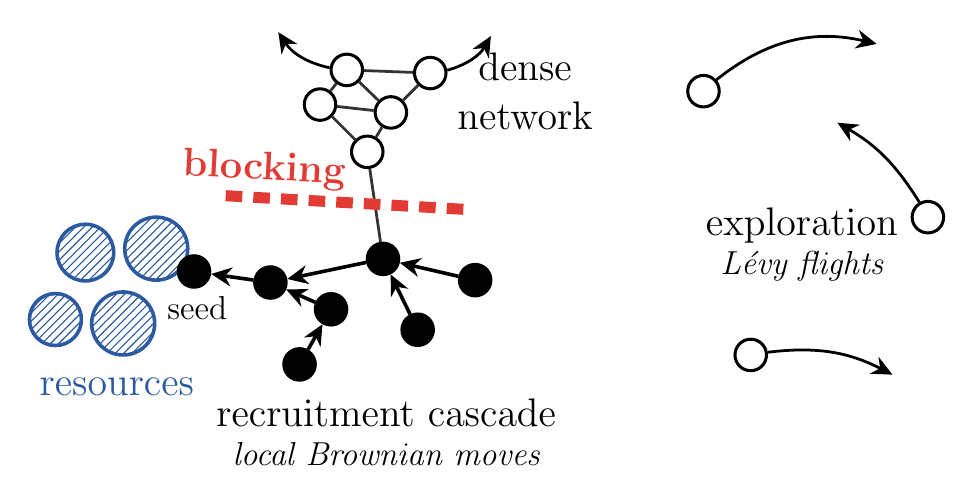
\begin{tikzpicture}[
    xscale=-1,                                   % <-- horizontal mirror of all geometry
    >={Stealth[length=2.6mm,width=2.4mm]},
    ag/.style={circle,draw=black,line width=1.1pt,fill=white,inner sep=0pt,minimum size=4.0mm},
    bd/.style={circle,draw=black,line width=1.1pt,fill=black,inner sep=0pt,minimum size=4.0mm},
    levy/.style={->,line width=1.0pt},          % curved long "hop"
    edge/.style={->,line width=1.3pt},
    net/.style={line width=1.0pt,black!80}]

  \definecolor{res}{HTML}{2C5AA0}
  \definecolor{blk}{HTML}{E23B33}

  % ---------------- exploration = curved, varying-length Levy hops (all black), nudged to new spots ----------------
  \node[ag] (e1) at (3.55,3.95) {}; \draw[levy] (e1) to[bend right=26] (1.35,4.55);  % long
  \node[ag] (e2) at (0.70,2.35) {}; \draw[levy] (e2) to[bend left=14]  (1.85,3.55);   % aimed UP, clear of text
  \node[ag] (e3) at (2.95,0.60) {}; \draw[levy] (e3) to[bend right=17] (1.15,0.35);   % medium-long
  \node[align=center,text=black] at (2.3,2.0) {{\Large exploration}\\[2pt]{\itshape\large L\'evy flights}};

  % ---------------- clumped resource (separate but clustered patches) + seed ----------------
  \foreach \cx/\cy/\s in {10.50/1.95/0.80, 11.40/1.90/0.72, 10.92/1.00/0.80, 11.78/1.05/0.66}{
    \node[circle,draw=res,line width=1.3pt,pattern=north east lines,pattern color=res,
          minimum size=\s cm,inner sep=0pt] at (\cx,\cy) {};
  }
  \node[res,font=\Large] at (11.0,0.2) {resources};
  \node[bd] (seed) at (10.02,1.66) {};                     % touches the leftmost resource patch
  \node[font=\large,anchor=north] at (9.98,1.47) {seed};   % label hugging just below the seed node

  % ---------------- recruitment cascade (filled dots converging on the seed), dots at new coords ----------------
  \node[bd] (f1) at (6.45,1.55) {};
  \node[bd] (g1) at (7.62,1.82) {};
  \node[bd] (m)  at (9.05,1.52) {};
  \node[bd] (f2) at (7.18,0.92) {};
  \node[bd] (g2) at (8.28,1.18) {};
  \node[bd] (f3) at (8.68,0.48) {};

  % ---------------- dense network (empty nodes), re-clustered into a new arrangement ----------------
  \node[ag] (n1) at (7.02,4.18) {};
  \node[ag] (n2) at (8.08,4.22) {};
  \node[ag] (n3) at (7.52,3.68) {};
  \node[ag] (n4) at (8.42,3.78) {};
  \node[ag] (n5) at (7.82,3.18) {};

  % edges: network graph, cascade tree, and ONE cross-link (cascade tries to grow into the clump)
  \draw[net] (n1)--(n2) (n1)--(n3) (n2)--(n3) (n2)--(n4) (n3)--(n4) (n3)--(n5) (n4)--(n5);
  \draw[net] (n5) -- (g1);                                  % the link that gets blocked
  \draw[edge] (f1) -- (g1);
  \draw[edge] (f2) -- (g1);
  \draw[edge] (f3) -- (g2);
  \draw[edge] (g2) -- (m);
  \draw[edge] (g1) -- (m);
  \draw[edge] (m)  -- (seed);

  % escaping (blocked) agents disperse via new long hops (bends flipped)
  \draw[levy] (n1) to[bend left=22]  (6.25,4.65);
  \draw[levy] (n2) to[bend right=22] (8.95,4.70);

  % ---------------- labels tied to their referents ----------------
  \node[align=center,font=\Large,anchor=west] at (6.80,3.95) {dense\\network};
  % recruitment cascade labelled directly BELOW its dots
  \node[align=center,anchor=north,text=black] at (7.58,0.17)
        {{\Large recruitment cascade}\\[2pt]{\itshape\large local Brownian moves}};

  % blocking bar in the gap between the dense-network nodes and the cascade, cutting n5--g1;
  % label in RED riding just above the line (angle adjusted for the mirrored geometry)
  \draw[blk,line width=4pt,dash pattern=on 6pt off 4pt] (6.6,2.45) -- (9.75,2.63);
  \node[font=\Large\bfseries,blk,anchor=south,rotate=-3] at (9.15,2.605) {blocking};

\end{tikzpicture}
\end{document}
